\chapter{Proposed Methodology}
\label{chap3}
In the previous chapter, we have discussed the theories that support this research related to the Electronic Voting Machine . In this chapter we will proposed our methodology for this project.
\section{Block Diagram}
Let us look at the simplified block diagram in Figure \ref{blockDiagram}, which illustrates the main components involved
in Electronic Voting Machine(EVM) Using 8051 Micro-controller. Switches are used to make choices, resister, capacitor, and oscillator are being used to work the micro-controller properly on the circuits with the help of connecting wires.
\begin{figure}[H]  %h=positioning
\begin{center}
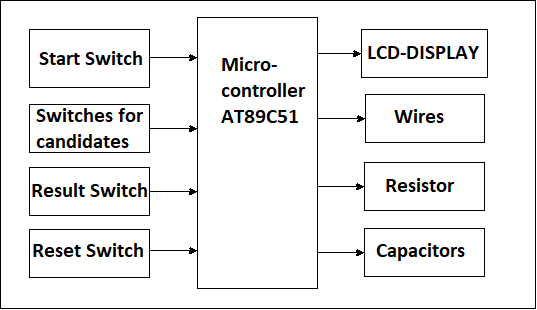
\includegraphics[scale=0.80]{Chapter3/blockDiagram}
\caption{Simplified Block Diagram of Electronic Voting Machine(EVM) Using 8051 Microcontroller}
\label{blockDiagram}
\end{center}
\end{figure}
\section{About Microcontroller 8051}
\noindent The 8051 Microcontroller was designed in the 1980s by Intel. Its foundation was on Harvard Architecture and was developed principally for bringing into play Embedded Systems. At first, it was created using NMOS technology but as NMOS technology needs more power to function therefore Intel re-intended Microcontroller 8051 employing CMOS technology and a new edition came into existence with a letter �C� in the title name, for illustration: 80C51. These most modern Microcontrollers need a fewer amount of power to function in comparison to their forerunners. There are many applications with an 8051 microcontroller.\\\\



\noindent The AT89C51 is a CMOS 8-bit microcomputer with 4K bytes of Flash programmable and erasable read only memory (PEROM).  The on-chip Flash allows the program memory to be reprogrammed in-system or by a ordinary nonvolatile memory programmer. Atmel AT89C51 is a powerful microcomputer/microcontroller (as they are used inter-changeably) which provides a highly-flexible and cost-effective solution to many embedded control applications.
\subsection{Features of AT89C51}
Following are some of the main feature of the used microcontroller i.e, AT89C51:
\begin{enumerate}
\item 8-bit CPU through two Registers A and B.
\item 8K Bytes � Internal ROM and it is a flash memory that supports while programming the system.
\item 256 Bytes � Internal RAM where the first RAM with 128 Bytes from 00H to 7FH is once more separated into four banks through 8 registers in every bank, addressable registers -16 bit \& general-purpose registers � 80.
\item The remaining 128 bytes of the RAM from 80H to FFH include Special Function Registers (SFRs). 
\item These registers control various peripherals such as Serial Port, Timers, all I/O Ports, etc.
\item Interrupts like External-2 \& Internal-3
\item Oscillator \& CLK Circuit.
\item Control Registers like PCON, SCON, TMOD, TCON, IE, and IP.
\item 16-bit Timers or Counters -2 like T0 \& T1.
\item Program Counter � 16 bit \& DPRT (Data Pointer).
\item I/O Pins � 32 which are arranged like four ports such as P0, P1, P2 \& P3.
\item Stack Pointer (SP) � 8bit \& PSW (Processor Status Word).
\item Serial Data Tx \& Rx for Full-Duplex Operation
\item a five vector two-level interrupt architecture
\item a full duplex serial port, on-chip oscillator and clock circuitry
%
\end{enumerate}
\section{Detailed Block Diagram - 8051}
Following is the detailed block diagram of the 8051.
\begin{figure}[H]  %h=positioning
\begin{center}
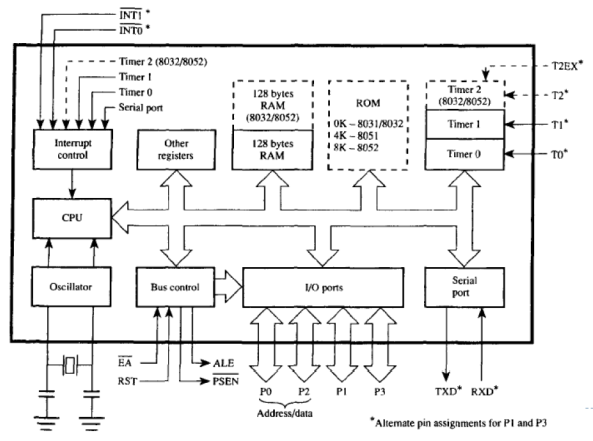
\includegraphics[scale=0.80]{Chapter3/blockDiagram8051}
\caption{Detailed Block Diagram of 8051 Microcontroller}
\label{blockDiagram8051}
\end{center}
\end{figure}
\subsection{Central Processor Unit (CPU)}
\noindent CPU is the brain of any processing device. It monitors and controls all operations that are performed in the Microcontroller. User has no control over the work of CPU. It reads program written in ROM memory and executes them and do the expected task.
\subsection{Interrupts}
\noindent Interrupt is a subroutine call that interrupts Microcontroller's main operation or work and causes it to execute some another program which is more important at that time. The feature of Interrupt is very useful as it helps in cases of emergency. Interrupts gives us a mechanism to put on hold the ongoing operation , execute a subroutine and then again resumes normal program execution The Microcontroller 8951 can be configured in such a way that it temporarily terminates or pause the main program at the occurrence of interrupt. When subroutine is completed then the execution of main program starts as usual. There are five interrupt sources in 8951 Microcontroller. 2 of them are external interrupts, 2 timer interrupts and one serial port interrupt.
\subsection{Input/output Port}
\noindent Microcontroller is used in embedded systems to control the operation of machines. Therefore to connect it to other machines, devices or peripherals we require I/O interfacing ports in Microcontroller. For this purpose Microcontroller 8951 has 4 input output ports to connect it to other peripherals.
Timers/Counters: Microcontroller 8951 has 2 16 bit timers and counters. The counters are divided into 8 bit registers. The timers are used for measurement of intervals, to determine pulse width etc.
\subsection{Oscillator}
\noindent Microcontroller is a digital circuit device, therefore it requires clock for its operation. For this purpose, Microcontroller 8951 has an on-chip oscillator which works as a clock source for Central Processing Unit. As the output pulses of oscillator are stable therefore it enables synchronized work of all parts of 8951 Microcontroller.
\subsection{Bus}
\noindent Basically Bus is a collection of wires which work as a communication channel or medium for transfer of Data. These buses consist of 8, 16 or more wires. Thus these can carry 8 bits, 16 bits simultaneously. Buses are of two types:
\begin{itemize}
\item Address Bus
%
\item Data Bus
%
\end{itemize}
\subsubsection{Address Bus}
Microcontroller 8051 has a 16 bit address bus. It used to address memory locations. It is used to transfer the address from CPU to Memory.
\subsubsection{Data Bus}
Microcontroller 8051 has 8 bits data bus. It is used to carry data.

\section{Pin Description 8051}
Following is the pin description diagram of the 8051
\begin{figure}[H]  %h=positioning
\begin{center}
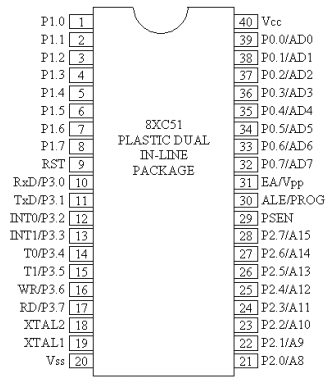
\includegraphics[scale=1.2]{Chapter3/pinDiagram}
\caption{Pin Diagram of 8051 Microcontroller}
\label{pinDiagram}
\end{center}
\end{figure}
\begin{figure}[H]  %h=positioning
\begin{center}
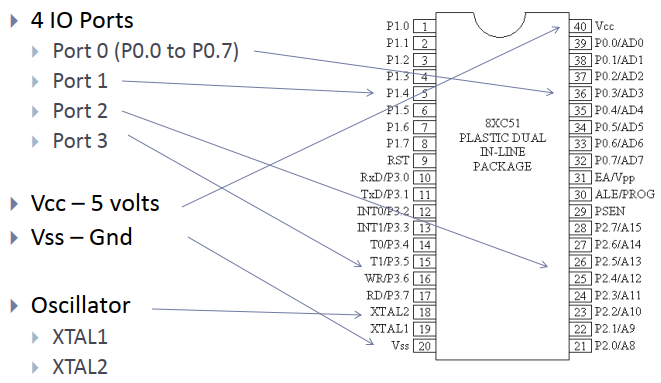
\includegraphics[scale=0.99]{Chapter3/pin1}
%\caption{Pin Diagram of 8051 Microcontroller}
%\label{pinDiagram}
\end{center}
\end{figure}
\begin{figure}[H]  %h=positioning
\begin{center}
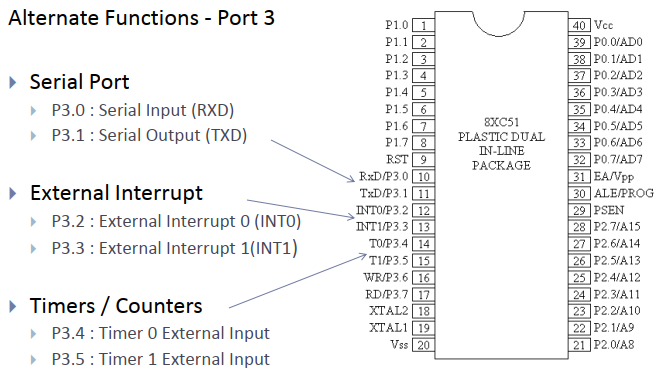
\includegraphics[scale=1.0]{Chapter3/pin2}
%\caption{Pin Diagram of 8051 Microcontroller}
%\label{pinDiagram}
\end{center}
\end{figure}
\begin{figure}[H]  %h=positioning
\begin{center}
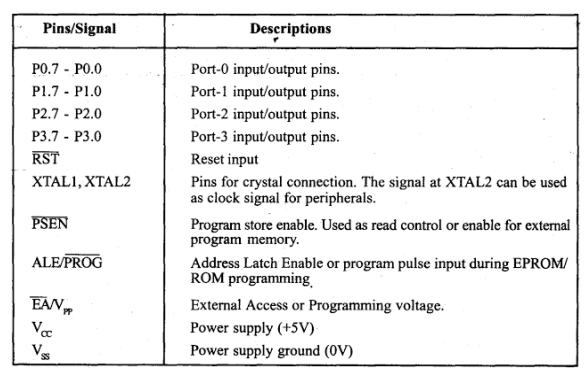
\includegraphics[scale=0.95]{Chapter3/pinsDetails}
\caption{Signals of 8031/8051 microcontroller of 8051 Microcontroller}
\label{pinsDetails}
\end{center}
\end{figure}
\begin{figure}[H]  %h=positioning
\begin{center}
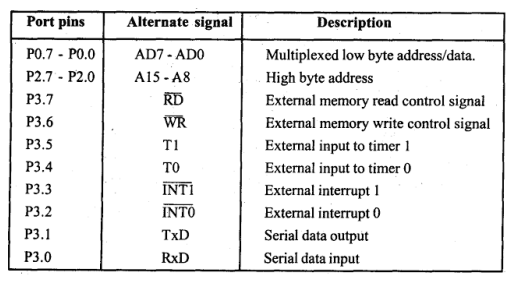
\includegraphics[scale=1.2]{Chapter3/pinsDetails1}
\caption{Alternate functions of port pins of 8051 Microcontroller}
\label{pinsDetails1}
\end{center}
\end{figure}

\subsection{Ports: (pin 1 to 8, pin 10 to 17, pin 21 to 28 and pin 32 to 39)}
\begin{itemize}
\item The 8031/8051 microcontroller has 32 I/O pins and they are organized as four numbers of 8-bit parallel
port.
\item The ports are denoted as port-0, port-1, port-2 and port-3. Each port can be used as either 8-bit parallel
port or 8 numbers of 1-bit ports.
\item The ports behave as latches during output operation and behave as buffers during input operation.
\item Port-1 can be used only for I/O operation
\item When external memory is employed, the port-0 function as multiplexed low byte address or data lines,
and port-2 function as high byte address lines. Therefore for accessing external memory the microcontroller
uses 16-bit address and access the memory in bytes. Hence the addressable memory space is 64 kb (216 =
64kb).
\item The 8031/8051 allows the external memory to be organized as two banks of 64 kb. One is program/code
memory and the other is data memory.
\end{itemize}
\subsection{PSEN (low signal): pin 29}
\begin{itemize}
\item The signal PSEN (low) is used as read control/enable for program memory.
RD (low signal) and WR (low signal): pin 17 and pin 16
\item The port pin P3.7 function as read control and the port pin P3.6 function as write control for data
memory.
\item When two external memory banks are not desirable, the PSEN (low) and RD (low) should be externally
ANDed to provide a single read control signal. In such cases the controller will access a common memory
space (of maximum capacity 64 kb) for program and data.
\item ALE is used to demultiplex the low byte address or data using an external latch.
\end{itemize}
\subsection{EA (Low)/Vpp : pin 31}
\begin{itemize}
\item When the microcontroller access program from external memory, then this pin is low. ie. EA (low) is
enabled.
\item When the microcontroller access program from internal memory, then this pin is high. At that time this
pin is used to supply programming voltage +12V to EPROM/ROM.
\end{itemize}
\subsection{XTAL 1 AND XTAL2: PIN 19 AND PIN18}
\begin{itemize}
\item The XTAL 1 and XTAL2 pins are provided for external quartz crystal connection, in order to generate the
required clock for the microcontroller. The maximum frequency of quartz crystal that can be connected to
8031/8051 microcontroller is 12 MHz.
\end{itemize}

\subsection{RST (low): pin 9}
\begin{itemize}
\item The RST(low) signal is used to reset the microcontroller in order to bring the controller to a known state.
\end{itemize}

\subsection{INTERRUPTS: pin 12 to 15}
\begin{itemize}
\item The 803 1/8051 has five interrupts.
\item In this two interrupts are external interrupt as INT0 (Low), INT1 (Low) and the remaining three are
internal interrupts as timer-0, timer-1 and serial port.
\item All interrupts are maskable and vectored interrupts.
\end{itemize}
\section{Components Selection}
\subsection{Hardware Components}
Following is the components which we have used to implement Electronic Voting Machine(EVM) Using 8051 Microcontroller.
\begin{figure}[H]  %h=positioning
\begin{center}
\includegraphics[scale=0.95]{Chapter3/comp1}
%\caption{Simplified Block Diagram of Electronic Voting Machine(EVM) Using 8051 Microcontroller}
%\label{blockDiagram}
\end{center}
\end{figure}
\begin{figure}[H]  %h=positioning
\begin{center}
\includegraphics[scale=0.95]{Chapter3/comp2}
%\caption{Simplified Block Diagram of Electronic Voting Machine(EVM) Using 8051 Microcontroller}
%\label{blockDiagram}
\end{center}
\end{figure}


\subsection{Software Selection}
To simulate our project, we have used proteus, the Proteus Design Suite is a proprietary software tool suite used primarily for electronic design automation. The software is used mainly by electronic design engineers and technicians to create schematics and electronic prints for manufacturing printed circuit boards. \begin{figure}[H]  %h=positioning
\begin{center}
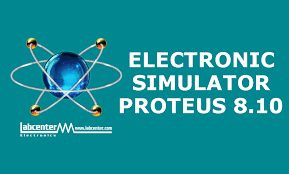
\includegraphics[scale= 1.5]{Chapter3/proteus}
%\caption{Simplified Block Diagram of Electronic Voting Machine(EVM) Using 8051 Microcontroller}
%\label{blockDiagram}
\end{center}
\end{figure}
